\documentclass[tikz,border=14pt]{standalone}
\usepackage[T1]{fontenc}
\usepackage{tgheros}
\usepackage{sfmath}
\usepackage{amsmath}
\usepackage{tikz}
\usetikzlibrary{arrows.meta,positioning,shapes.geometric,fit,backgrounds,calc}
\usepackage{xcolor}

\renewcommand{\familydefault}{\sfdefault}

% Harvard Crimson & ETH Zurich Academic Semantic Palette
\definecolor{crimson}{HTML}{A51C30}
\definecolor{navy}{HTML}{1F407A}
\definecolor{blueaccent}{HTML}{215CAF}
\definecolor{petrol}{HTML}{007A87}
\definecolor{bronze}{HTML}{B87333}
\definecolor{purple}{HTML}{5B4B8A}
\definecolor{darkslate}{HTML}{0F172A}
\definecolor{slate}{HTML}{475569}
\definecolor{muted}{HTML}{64748B}
\definecolor{cardbg}{HTML}{FFFFFF}
\definecolor{subtlebg}{HTML}{F8FAFC}
\definecolor{cardborder}{HTML}{CBD5E1}

\begin{document}
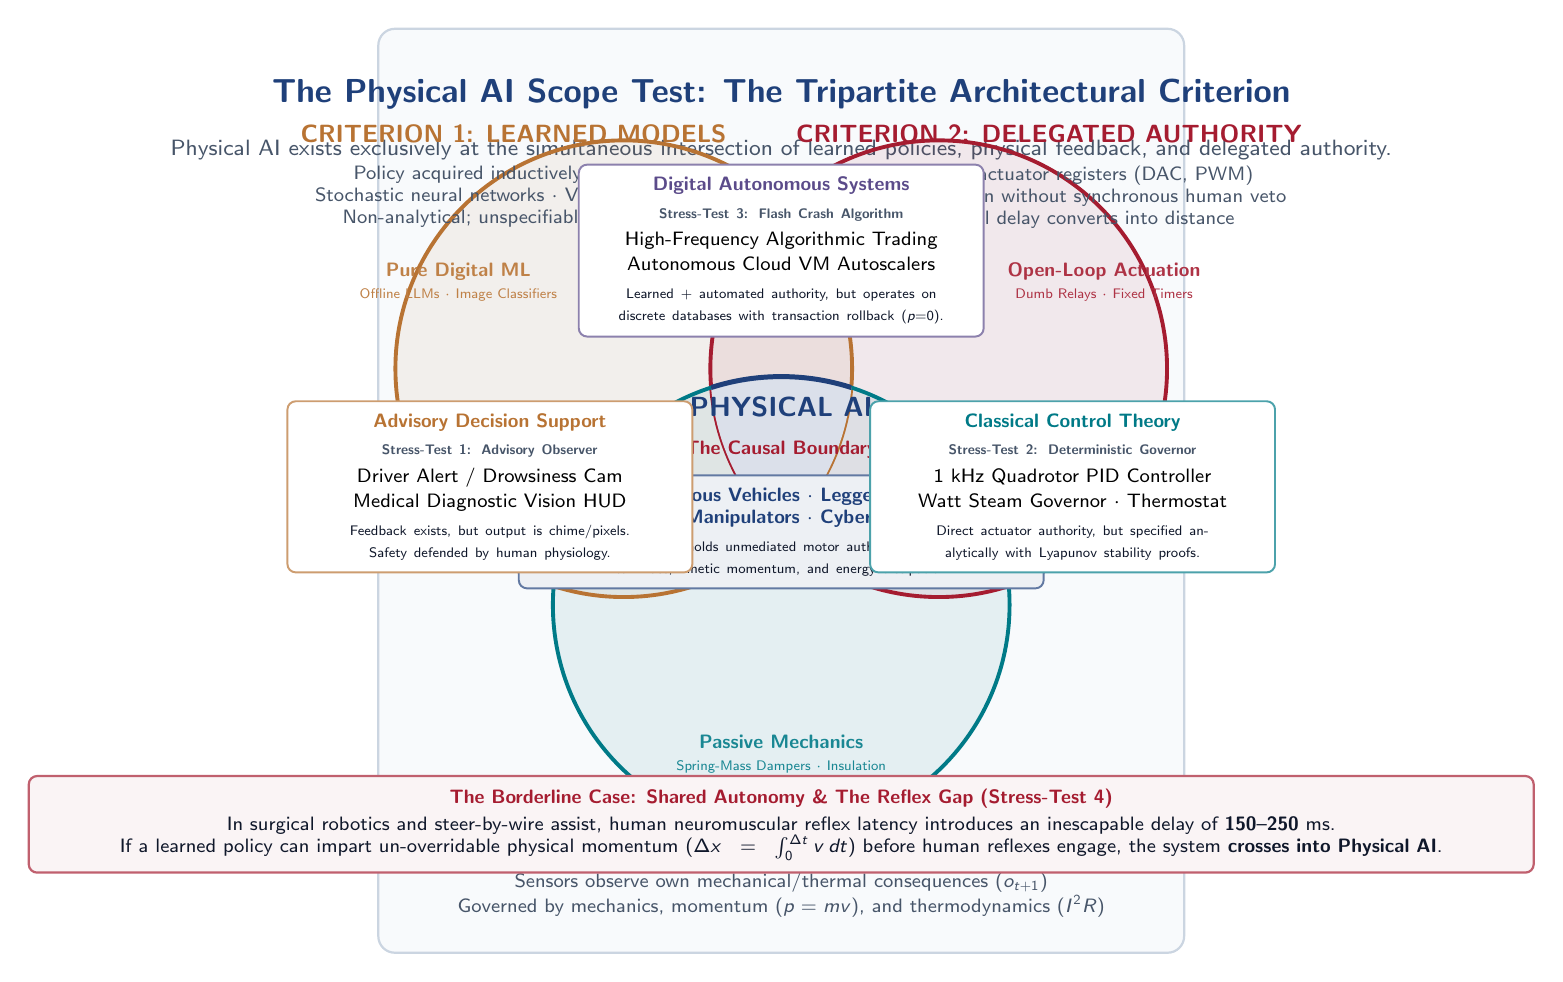
\begin{tikzpicture}[
  font=\sffamily,
  >=Stealth,
  annot/.style={
    font=\sffamily\scriptsize,
    text=darkslate,
    align=center
  },
  tagbox/.style={
    draw=cardborder,
    fill=white,
    rounded corners=3pt,
    line width=0.7pt,
    inner sep=4.5pt,
    align=center,
    font=\sffamily\scriptsize
  }
]

  % Title Banner
  \node[font=\sffamily\bfseries\large, text=navy, anchor=north] (title) at (0, 5.0) {
    The Physical AI Scope Test: The Tripartite Architectural Criterion
  };
  \node[font=\sffamily\footnotesize, text=slate, below=0.06in of title.south, anchor=north] (subtitle) {
    Physical AI exists exclusively at the simultaneous intersection of learned policies, physical feedback, and delegated authority.
  };

  % Define Circle Centers
  \coordinate (C_learned)   at (-2.0, 1.2);   % Top Left: Learned Models
  \coordinate (C_authority) at ( 2.0, 1.2);   % Top Right: Delegated Authority
  \coordinate (C_feedback)  at ( 0.0, -1.8);  % Bottom Center: Physical Feedback

  \def\R{2.9} % Circle Radius

  % --- Draw Filled Circles in Background ---
  \begin{scope}[fill opacity=0.08]
    \fill[bronze]   (C_learned)   circle (\R);
    \fill[crimson]  (C_authority) circle (\R);
    \fill[petrol]   (C_feedback)  circle (\R);
  \end{scope}

  % Draw Circle Outlines
  \draw[bronze, line width=1.4pt]  (C_learned)   circle (\R);
  \draw[crimson, line width=1.4pt] (C_authority) circle (\R);
  \draw[petrol, line width=1.4pt]  (C_feedback)  circle (\R);

  % --- Center Intersection Highlight (Physical AI) ---
  \begin{scope}
    \clip (C_learned) circle (\R);
    \clip (C_authority) circle (\R);
    \fill[navy!16] (C_feedback) circle (\R);
    \draw[navy, line width=1.8pt] (C_feedback) circle (\R);
  \end{scope}

  % =========================================================================
  % CIRCLE HEADERS / PRIMARY CRITERIA
  % =========================================================================

  % 1. Learned Models (Top Left)
  \node[font=\sffamily\bfseries\small, text=bronze, anchor=south] at (-3.4, 3.95) {
    CRITERION 1: LEARNED MODELS
  };
  \node[annot, text=slate, anchor=north] at (-3.4, 3.9) {
    Policy acquired inductively from data\\
    Stochastic neural networks $\cdot$ VLMs $\cdot$ Diffusion\\
    Non-analytical; unspecifiable edge cases
  };

  % 2. Delegated Physical Authority (Top Right)
  \node[font=\sffamily\bfseries\small, text=crimson, anchor=south] at (3.4, 3.95) {
    CRITERION 2: DELEGATED AUTHORITY
  };
  \node[annot, text=slate, anchor=north] at (3.4, 3.9) {
    Direct write to actuator registers (DAC, PWM)\\
    Automated execution without synchronous human veto\\
    Computational delay converts into distance
  };

  % 3. Physical Feedback (Bottom Center)
  \node[font=\sffamily\bfseries\small, text=petrol, anchor=north] at (0, -4.5) {
    CRITERION 3: CONSEQUENTIAL PHYSICAL FEEDBACK
  };
  \node[annot, text=slate, anchor=north] at (0, -4.8) {
    Actuator forces alter physical state ($W_t \to W_{t+1}$)\\
    Sensors observe own mechanical/thermal consequences ($o_{t+1}$)\\
    Governed by mechanics, momentum ($p=mv$), and thermodynamics ($I^2R$)
  };

  % =========================================================================
  % REGION LABELS & EXAMPLES
  % =========================================================================

  % CENTER: Physical AI (1 + 2 + 3)
  \node[font=\sffamily\bfseries\normalsize, text=navy, align=center] at (0, 0.45) (center_label) {
    PHYSICAL AI\\[2pt]
    {\scriptsize\color{crimson}\textbf{The Causal Boundary}}
  };
  \node[tagbox, draw=navy!70, fill=navy!8, below=0.03in of center_label, text width=2.5in] (center_box) {
    {\scriptsize\textbf{\color{navy}Autonomous Vehicles $\cdot$ Legged Robots}}\\
    {\scriptsize\textbf{\color{navy}Dexterous Manipulators $\cdot$ Cybernetic Loops}}\\[2pt]
    {\tiny\color{darkslate}Learned policy holds unmediated motor authority over physical mass, kinetic momentum, and energy dissipation.}
  };

  % INTERSECTION: Learned + Feedback, NO Authority (Advisory ML / Decision Support)
  \node[tagbox, draw=bronze!70, fill=white, text width=1.9in] at (-3.7, -0.3) {
    \textbf{\color{bronze} Advisory Decision Support}\\[2pt]
    {\tiny\color{slate}\textbf{Stress-Test 1: Advisory Observer}}\\[2pt]
    {\scriptsize Driver Alert / Drowsiness Cam}\\[1pt]
    {\scriptsize Medical Diagnostic Vision HUD}\\[2pt]
    {\tiny\color{darkslate}Feedback exists, but output is chime/pixels. Safety defended by human physiology.}
  };

  % INTERSECTION: Feedback + Authority, NO Learning (Classical Control)
  \node[tagbox, draw=petrol!70, fill=white, text width=1.9in] at (3.7, -0.3) {
    \textbf{\color{petrol} Classical Control Theory}\\[2pt]
    {\tiny\color{slate}\textbf{Stress-Test 2: Deterministic Governor}}\\[2pt]
    {\scriptsize 1 kHz Quadrotor PID Controller}\\[1pt]
    {\scriptsize Watt Steam Governor $\cdot$ Thermostat}\\[2pt]
    {\tiny\color{darkslate}Direct actuator authority, but specified analytically with Lyapunov stability proofs.}
  };

  % INTERSECTION: Learned + Authority, NO Physical Feedback (Digital Autonomy)
  \node[tagbox, draw=purple!70, fill=white, text width=1.9in] at (0, 2.7) {
    \textbf{\color{purple} Digital Autonomous Systems}\\[2pt]
    {\tiny\color{slate}\textbf{Stress-Test 3: Flash Crash Algorithm}}\\[2pt]
    {\scriptsize High-Frequency Algorithmic Trading}\\[1pt]
    {\scriptsize Autonomous Cloud VM Autoscalers}\\[2pt]
    {\tiny\color{darkslate}Learned + automated authority, but operates on discrete databases with transaction rollback ($p{=}0$).}
  };

  % =========================================================================
  % EXCLUSIVE OUTER REGIONS
  % =========================================================================

  \node[annot, text=bronze!90] at (-4.1, 2.3) {
    \textbf{Pure Digital ML}\\
    {\tiny Offline LLMs $\cdot$ Image Classifiers}
  };

  \node[annot, text=crimson!90] at (4.1, 2.3) {
    \textbf{Open-Loop Actuation}\\
    {\tiny Dumb Relays $\cdot$ Fixed Timers}
  };

  \node[annot, text=petrol!90] at (0, -3.7) {
    \textbf{Passive Mechanics}\\
    {\tiny Spring-Mass Dampers $\cdot$ Insulation}
  };

  % =========================================================================
  % BOTTOM CALLOUT: THE SHARED AUTONOMY REFLEX GAP
  % =========================================================================

  \node[tagbox, draw=crimson!70, fill=crimson!5, line width=0.8pt, text width=7.4in, align=center,
        below=0.85in of C_feedback, anchor=north] (reflex_callout) {
    \textbf{\color{crimson} The Borderline Case: Shared Autonomy \& The Reflex Gap (Stress-Test 4)}\\[2pt]
    {\scriptsize\color{darkslate}In surgical robotics and steer-by-wire assist, human neuromuscular reflex latency introduces an inescapable delay of $\mathbf{150\text{--}250\text{ ms}}$.}\\
    {\scriptsize\color{darkslate}If a learned policy can impart un-overridable physical momentum ($\Delta x = \int_0^{\Delta t} v \, dt$) before human reflexes engage, the system \textbf{crosses into Physical AI}.}
  };

  % Coordinate anchors for background bounding box
  \coordinate (b_top_left) at (-5.0, 5.4);
  \coordinate (b_bot_right) at (5.0, -6.1);

  % Background container
  \begin{scope}[on background layer]
    \node[draw=cardborder, fill=subtlebg, rounded corners=6pt, line width=0.8pt,
          fit=(b_top_left) (b_bot_right)] (bounding_box) {};
  \end{scope}

\end{tikzpicture}
\end{document}
